\begin{frame}{Desenvolvimento do site}
\framesubtitle{Organização}
O projeto foi estruturado em 4 seções principais: O site principal, a vitrine de artistas, os editais e escola de artes. Cada seção foi desenhada com foco em acessibilidade e usabilidade.

\vspace{\baselineskip}

\begin{center}
    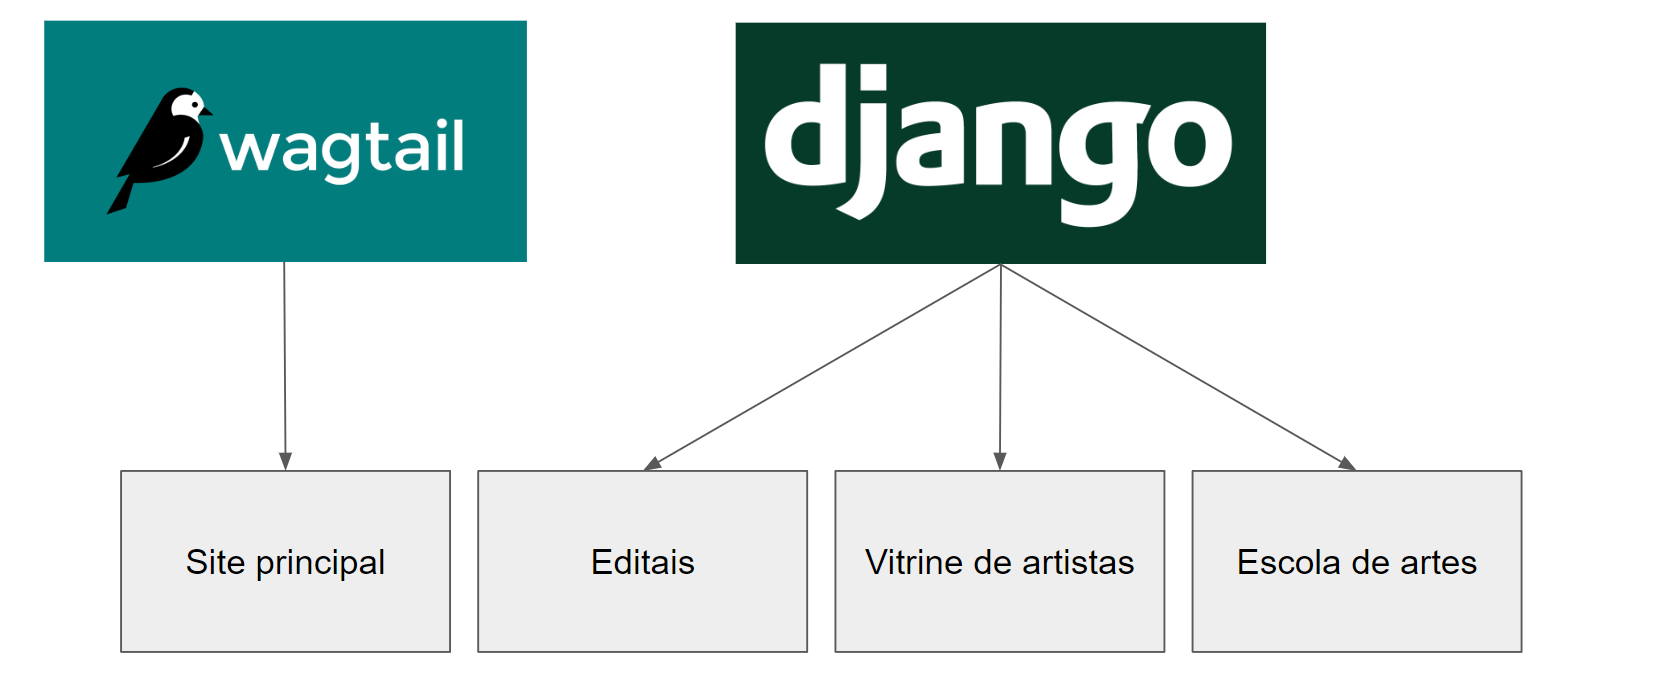
\includegraphics[height=0.65\textheight]{beamerthemesrc/assets/organizacao.png}
\end{center}

\end{frame}

\begin{frame}{Vitrine de artistas}
\framesubtitle{Modelo de dados}

Cada artista poderia ter informações como Nome, Nome Artístico, Área de Atuação,
Links para portfólios ou redes sociais, documentos, imagens e uma categorização por área
de atuação
    
\end{frame}

\begin{frame}{Vitrine de artistas}
\framesubtitle{Modelo de dados}

    \begin{center}
        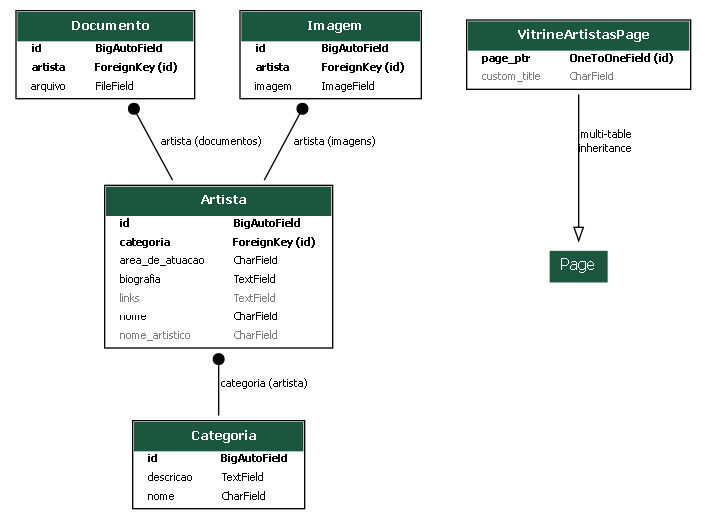
\includegraphics[height=\textheight]{beamerthemesrc/assets/er_diagram_vitrine.png}
    \end{center}

\end{frame}

\begin{frame}{Vitrine de artistas}
\framesubtitle{Site principal}
    O site possui uma página exclusiva para a vitrine de artistas.
    
    \vspace{\baselineskip}
    
        \begin{center}
            
\includegraphics[width=\textwidth]{beamerthemesrc/assets/vitrine_de_artistas.png}
        \end{center}
\end{frame}
    
\begin{frame}{Vitrine de artistas}
\framesubtitle{Site principal}
    Também é possível o cadastramento através de um formulário no site.
    
    \vspace{\baselineskip}
    
        \begin{center}
            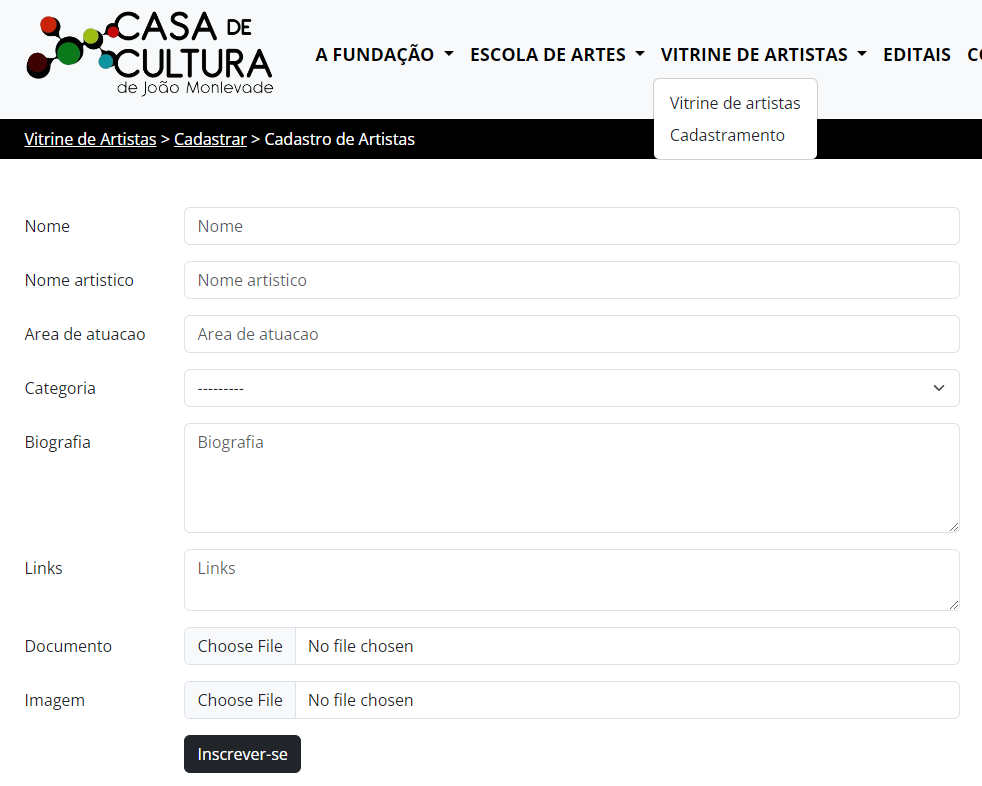
\includegraphics[scale=0.25]{beamerthemesrc/assets/form_artista.png}
        \end{center}
\end{frame}

\begin{frame}{Vitrine de artistas}
\framesubtitle{Site administrativo}
\textbf{Funcionalidades do administrador:}

\begin{itemize}
    \item Criar, editar e deletar um artista.
    \item Aprovar a publicação de um artista na vitrine.
\end{itemize}
    
    \vspace{\baselineskip}
    
        \begin{center}
            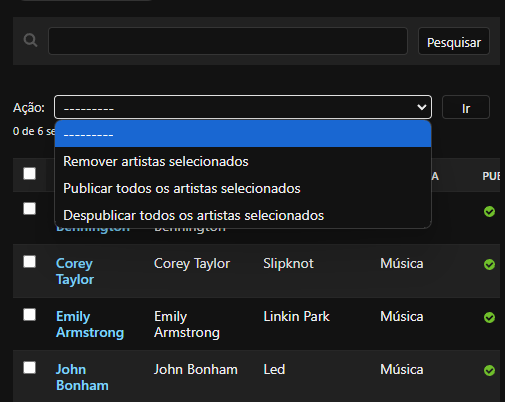
\includegraphics[scale=0.4]{beamerthemesrc/assets/admin_artista.png}
        \end{center}
\end{frame}


\begin{frame}{Editais}
\framesubtitle{Modelo de dados}

Cada edital possui um título, uma descrição detalhada,
uma categoria, um período de inscrição definido por uma data e hora de início e término,
e um status que pode ser "Aberto", "Fechado"ou "Indisponível".

\end{frame}

\begin{frame}{Editais}
\framesubtitle{Modelo de dados}

    \begin{center}
        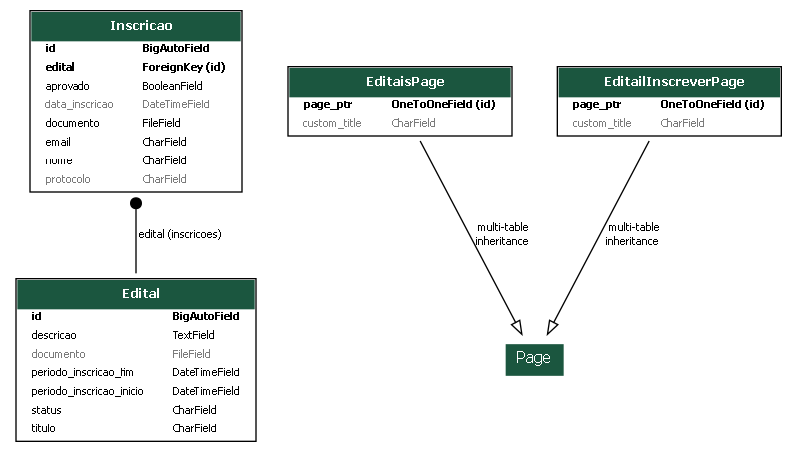
\includegraphics[height=\textheight]{beamerthemesrc/assets/er_diagram_editais.png}
    \end{center}

    
\end{frame}

\begin{frame}{Editais}
    \framesubtitle{Site administrativo}
    \textbf{Funcionalidades do administrador:}

    \begin{itemize}
        \item Criar, editar e deletar editais.
        \item Aprovar um candidato.
        \item Filtrar candidaturas.
    \end{itemize}
        
            \begin{center}
                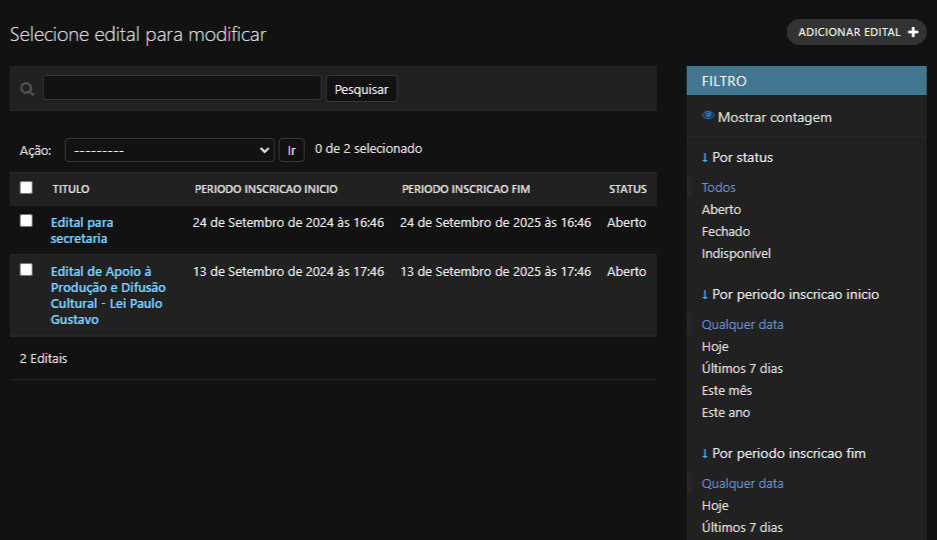
\includegraphics[scale=0.3]{beamerthemesrc/assets/admin_edital.png}
            \end{center}
\end{frame}

\begin{frame}{Editais}
\framesubtitle{Site principal}
    O visitante pode visualizar os editais e se candidatar aos que estão abertos através de uma página própria com formulário.
    
    \vspace{\baselineskip}
    
        \begin{center}
            
\includegraphics[scale=0.18]{beamerthemesrc/assets/lista_editais.png}
            
\includegraphics[scale=0.15]{beamerthemesrc/assets/form_edital.png}
        \end{center}
\end{frame}


\begin{frame}{Escola de artes}
\framesubtitle{Modelo de dados}

    A base do modelo são as Turmas, associadas a um Curso e a um Professor, que podem ter vários Alunos.
    
    \vspace{\baselineskip}
    
    Para registrar ocorrências, acompanhar a frequência e a pontuação dos alunos,
    foram criados os modelos Ocorrência, Frequência e Pontuação.
    
\end{frame}
    
\begin{frame}{Escola de artes}
\framesubtitle{Modelo de dados}

\begin{center}
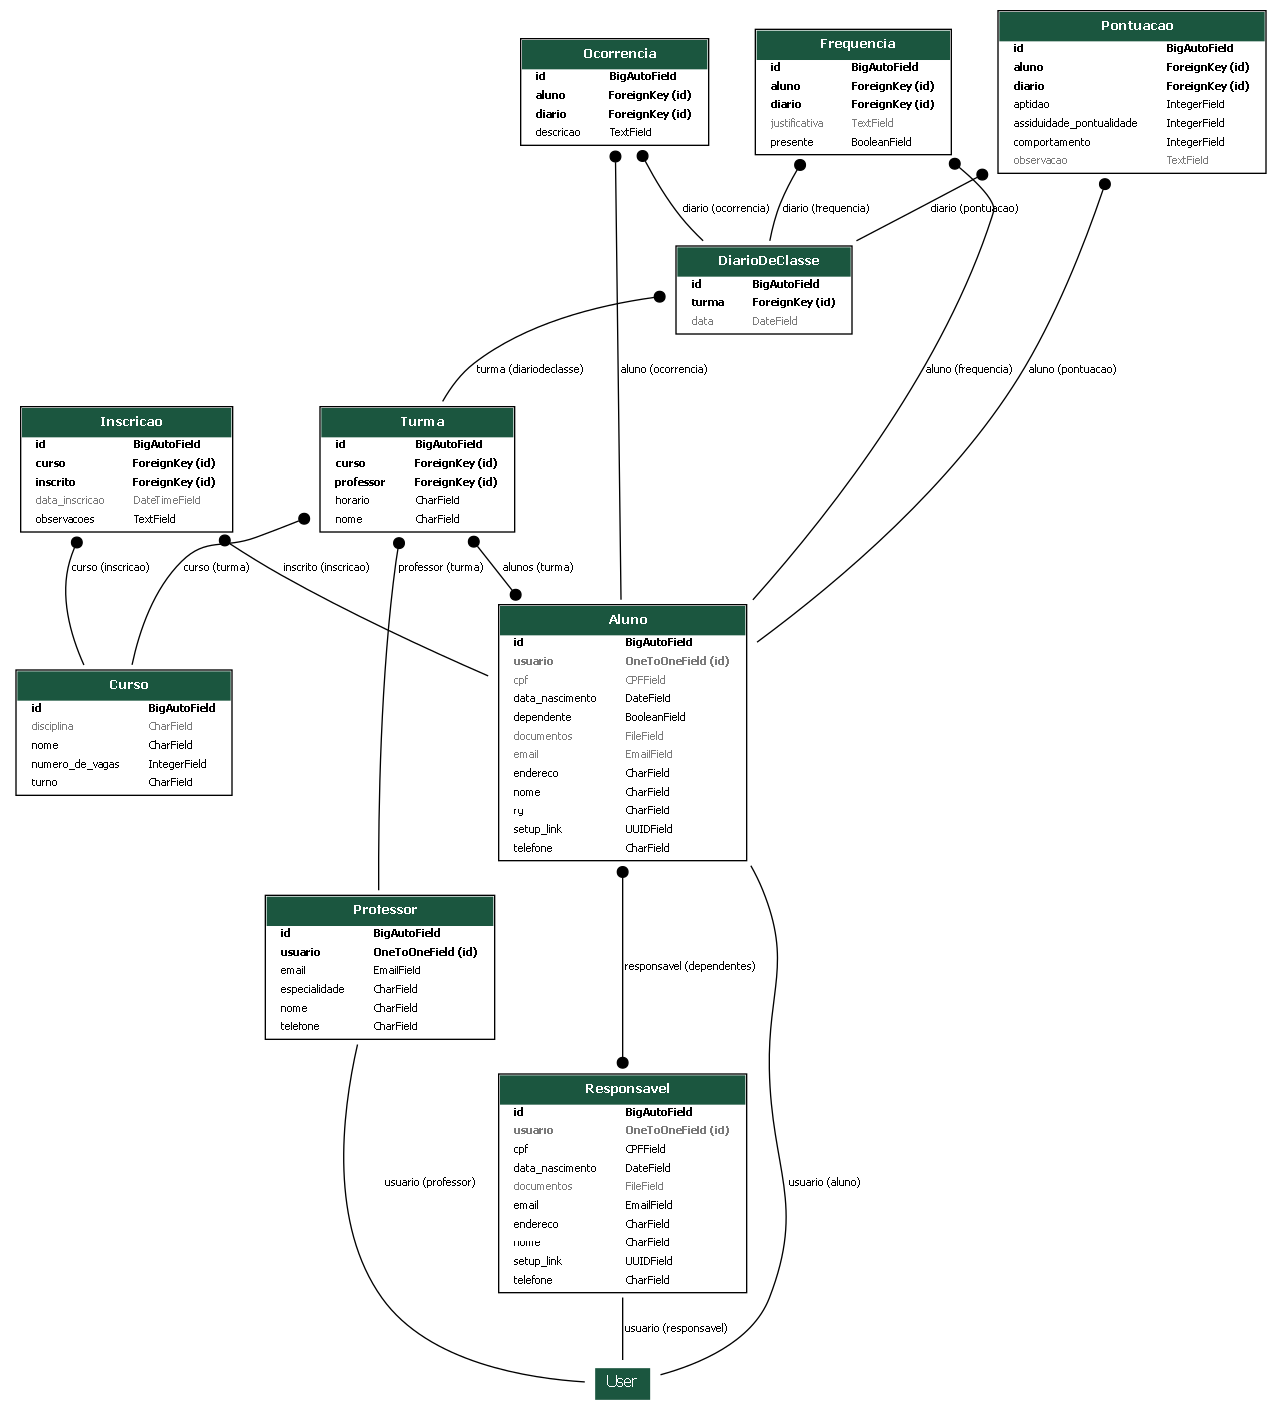
\includegraphics[height=\textheight]{beamerthemesrc/assets/er_diagram_escola.png}
\end{center}


\end{frame}

\begin{frame}{Escola de artes}
\framesubtitle{Modelo de dados}

\begin{center}
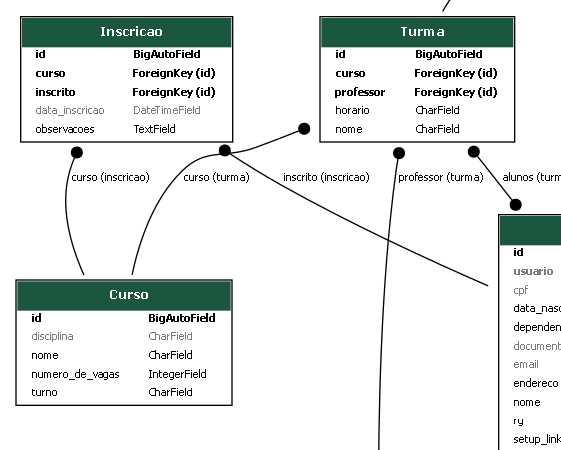
\includegraphics[height=\textheight]{beamerthemesrc/assets/er_diagram_escola_turma.png}
\end{center}


\end{frame}

\begin{frame}{Escola de artes}
\framesubtitle{Modelo de dados}

\begin{center}
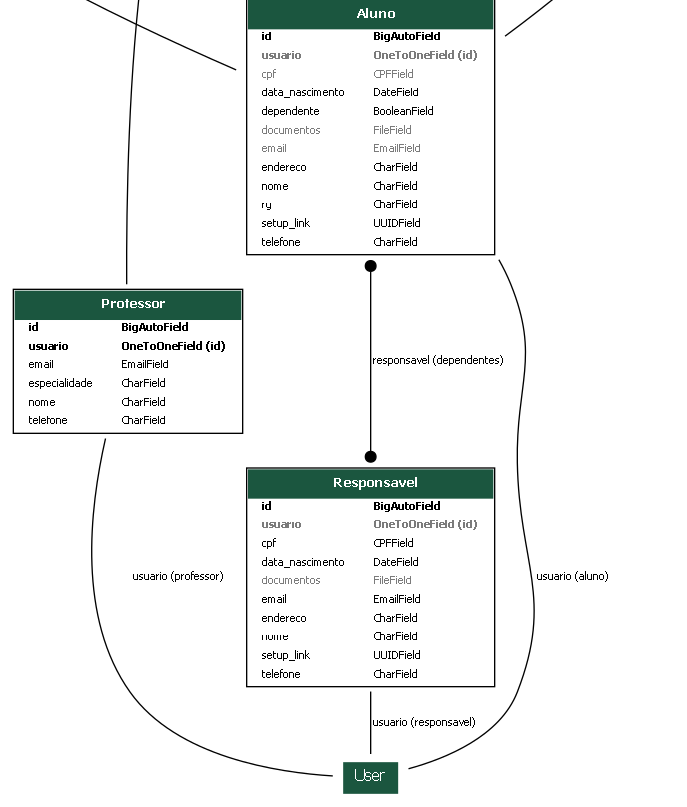
\includegraphics[scale=0.33]{beamerthemesrc/assets/er_diagram_escola_aluno.png}
\end{center}


\end{frame}

\begin{frame}{Escola de artes}
\framesubtitle{Modelo de dados}

\begin{center}
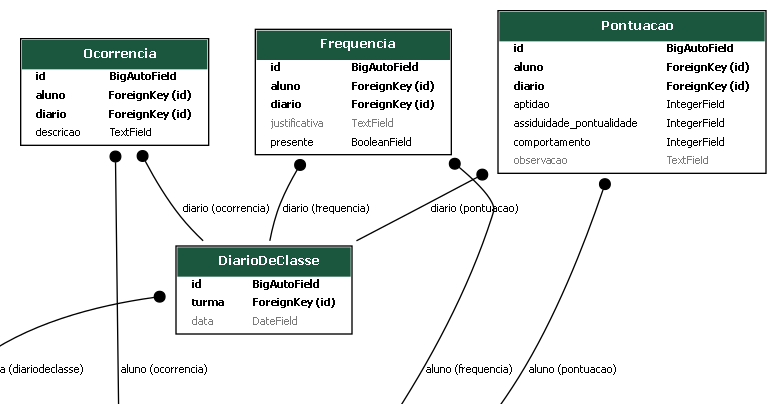
\includegraphics[height=\textheight]{beamerthemesrc/assets/er_diagram_escola_diario.png}
\end{center}


\end{frame}


\begin{frame}{Escola de artes}
    \framesubtitle{Site administrativo}
    \textbf{Funcionalidades do administrador:}

    \begin{itemize}
        \item Criar, editar e deletar cursos, turmas, alunos, professores e diários de classe.
        \item Criar usuários e gerar o link de criação de senha.
    \end{itemize}

\end{frame}

\begin{frame}{Escola de artes}
    \framesubtitle{Site administrativo}
    \textbf{Funcionalidades do professor:}

    \begin{itemize}
        \item Criar, editar e deletar ocorrências, pontuações, frequências e diários de classe.
    \end{itemize}
        
        \vspace{\baselineskip}
        
            \begin{center}
                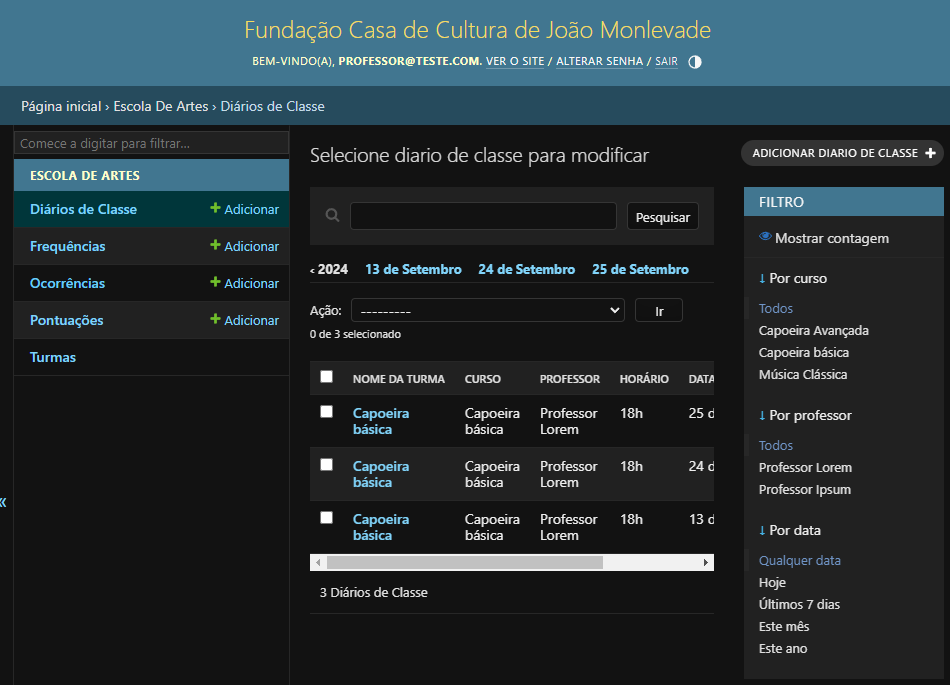
\includegraphics[scale=0.25]{beamerthemesrc/assets/admin_professor.png}
            \end{center}
\end{frame}

\begin{frame}{Escola de artes}
    \framesubtitle{Site administrativo}
    \textbf{Funcionalidades do aluno/responsável:}

    \begin{itemize}
        \item Visualizar apenas suas próprias ocorrências, pontuações e frequências.
    \end{itemize}

    \vspace{\baselineskip}
        
    \begin{center}
        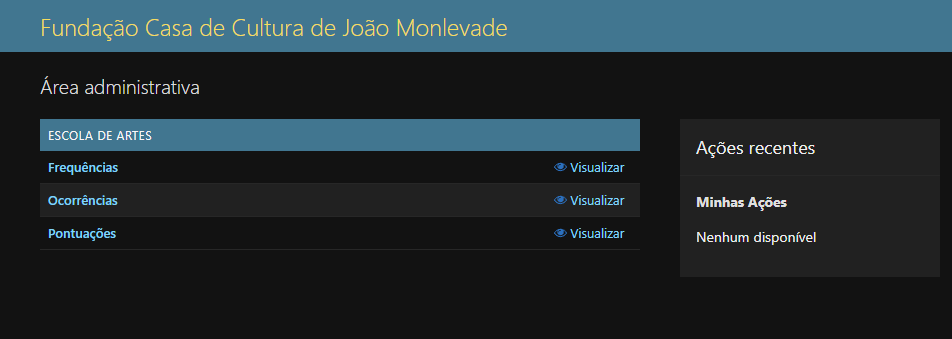
\includegraphics[scale=0.4]{beamerthemesrc/assets/admin_aluno.png}
    \end{center}
\end{frame}

\begin{frame}{Site principal}
\framesubtitle{Navbar e slider}
A página inicial funciona
como um resumo dinâmico do que está acontecendo na instituição, com links diretos para
as seções e notícias mais relevantes.

\vspace{\baselineskip}

    \begin{center}
        
\includegraphics[width=\textwidth]{beamerthemesrc/assets/pagina_principal.png}
    \end{center}
\end{frame}

\begin{frame}{Site principal}
\framesubtitle{Lista de artigos e rodapé}
A parte inferior da página lista os últimos artigos e o rodapé da possui links e informações uteis.  

\vspace{\baselineskip}

    \begin{center}
        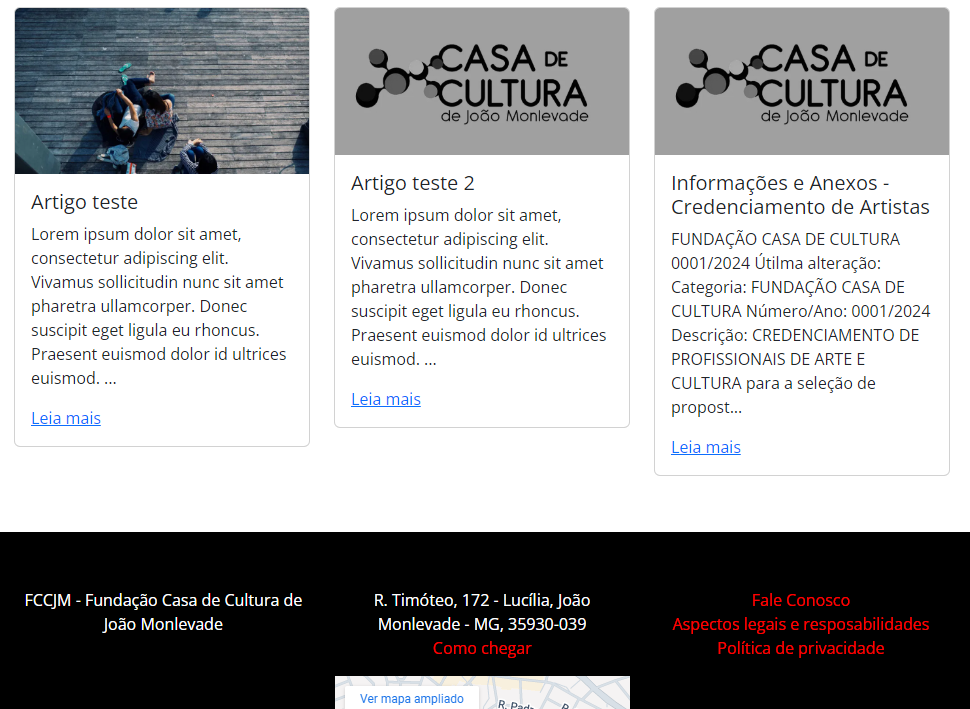
\includegraphics[scale=0.25]{beamerthemesrc/assets/artigos_footer.png}
    \end{center}
\end{frame}

\begin{frame}{Site principal}
\framesubtitle{Artigo}
Um artigo mostra as informações do autor, data e pode ter uma imagem. Também é possível ver a hierarquia do documento.

\vspace{\baselineskip}

    \begin{center}
        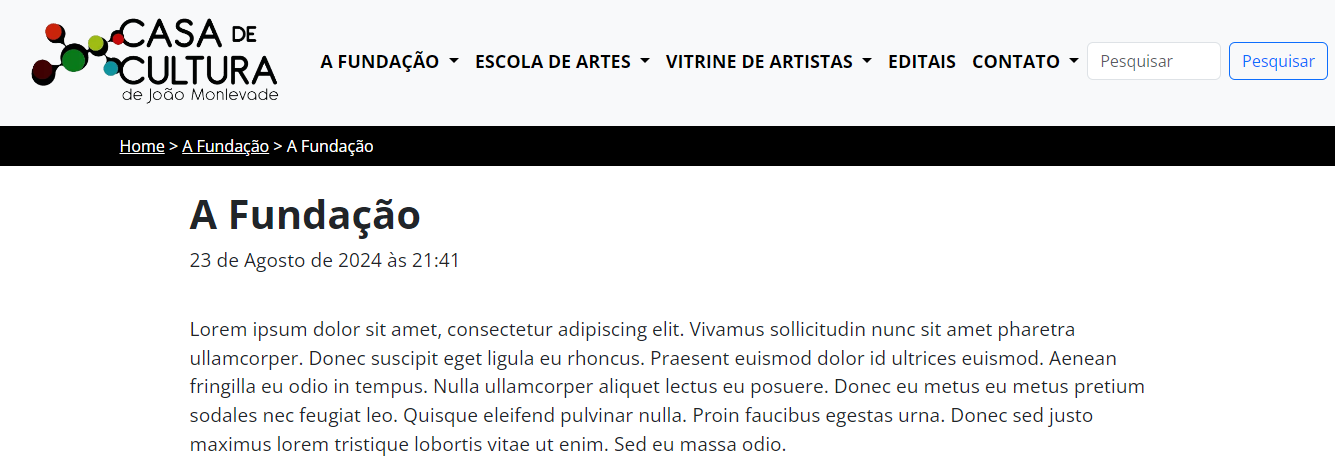
\includegraphics[width=\textwidth]{beamerthemesrc/assets/artigo.png}
    \end{center}
\end{frame}

\begin{frame}{Site principal}
    \framesubtitle{Responsividade}
    
        \begin{center}
            
\includegraphics[height=\textheight]{beamerthemesrc/assets/responsividade1.png}
            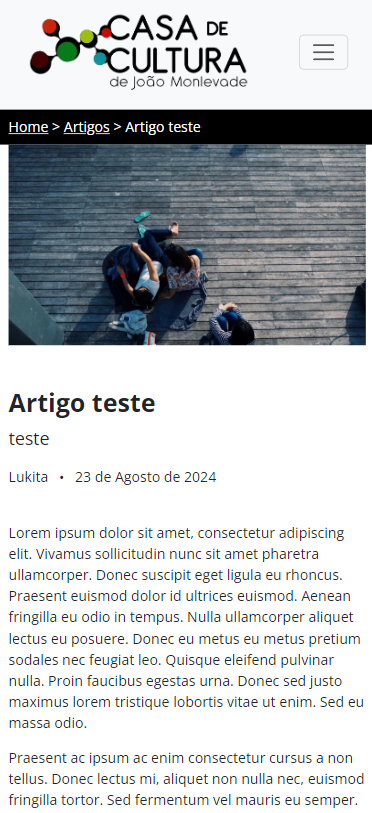
\includegraphics[height=\textheight]{beamerthemesrc/assets/responsividade2.png}
            
\includegraphics[height=\textheight]{beamerthemesrc/assets/responsividade3.png}
            
\includegraphics[height=\textheight]{beamerthemesrc/assets/responsividade4.png}
        \end{center}
    \end{frame}
